\documentclass{report}

\usepackage[utf8]{inputenc}
\usepackage[document]{ragged2e}
\usepackage{graphicx}
\graphicspath{ {C:/Users/alhan/Documents/projects/billeder/}}
\usepackage{Sweave}
\begin{document}
\Sconcordance{concordance:aflevering_reaflevering.tex:aflevering_reaflevering.Rnw:%
1 6 1 1 0 26 1 1 12 118 1 1 3 41 0 1 2 19 1 1 5 60 1 1 4 132 0 1 2 2 1 %
1 4 132 0 1 2 1 1}

\begin{titlepage}
    \begin{center}
        \vspace*{1cm}
 
        \Huge
        \textbf{Machine learning - DTU}
 
        \vspace{0.5cm}
        \LARGE
        Rapport 
 
        \vspace{1.5cm}
 
        \textbf{Anna Louise Hansen}
        \vfill
 
        Fra Udviklings- og Forenklingsstyrrelsen
 
        \vspace{0.8cm}
 
    \end{center}
\end{titlepage}

\chapter{Part I}


\section{Beskrivelse af data}
Alle boligejere i Danmark betaler en skat, ejendomsværdiskat, som er baseret på værdien af deres
ejendom. Dette vil sige værdien af hele ejendommen inkl. den grund som boligen ligger på. For at
kunne gøre dette laver den danske stat offentlige ejendomsvurderinger som disse skatter bliver
baseret på. 
Det er derfor vigtigt at disse vurderinger er retvisende og ikke mindst forklarbare, således at en
borger kan forstå hvilke parametre der ligger til grund for ejendomsvurderingen. 
Til dette project har jeg valgt at arbejde med anonymiseret data fra mit arbejde i udviklings- og
forenklingsstyrrelsen, hvor jeg til dagligt arbejder med netop dette. Datasættet består af
ejendomssalg fra en 6 årig periode. Ud over selve salgspriserne består data også af en lang række
attributter som beskriver karakteristika ved selve boligen. Det kan f.eks. være tagmateriale,
boligens opførelsesår, information om størrelsen af huset og grunden eller bbr koder som dækker
over boligens anvendelse. 
Der ud over består data også af en lang række attributter som fortæller noget om hvor boligens
beliggenhed. Det kan f.eks. være boligens koordinater, områdepriserne (baseret på de nærmeste
nabosalg) eller information om afstanden til kyst og skov eller afstand til motorvej og jernbane. 
Data kommer fra en række forskellige registre og offentlige styrrelser som eks. BBR og Styrrelsen
for Dataforsyning og Effektivisering.

Til dette projekt vil jeg overordnet set prøve at se hvor godt man kan forudsige ejendomsværdier 
ud fra salgspriserne fra en 6-årig periode. 

Jeg vil med Principal Component Analysis få et overblik over de data der er til rådighed og få et
visuelt overblik over attributterne. 
Herefter vil jeg med unsupervised learning forsøge at gruppere det data jeg har således at jeg ud
fra det kan generere yderlige attributter som kan indgå i modellen. Jeg vil her specifikt prøve at
se om det er muligt at gruppere salgene i forskellige boligtyper. Jeg vil i samme omgang også
forsøge at frasorterer outliers i data med anomaly detection. 
Herefter vil jeg med regressions model forsøge at kaste lys over projektets overordnede problem ved
at forsøge at forudsige huspriserne ud fra salgspriser. I tilfælde af at modellen ikke ikke kan
komme med en god prædiktion af en given ejendom vil det være muligt at denne ejendom bliver manuelt
værdiansat af en sagsbehandler. Jeg vil derfor til slut med en Klassifikationsmodel forsøge at
estimerer om en ejendom skal ud til manuel sagsbehandling baseret på dens estimerede ejendomsværdi.

\section{Detaljeret beskrivelse af data}

Det salgsdata som jeg har valgt at arbejde med dækker i udgangspunktet 305701 observationer med 126
attributter (se bilag 1). Inden jeg går i gang med at kigge på data har jeg valgt at lave en oprydning i data.
Mange af attributterne har ikke noget med selve ejendommen at gøre men er forretningsmæssige
oplysninger som ikke er relevante for denne opgave. Desuden dækker observationerne mange forskellig
e typer af ejendomssalg. Det er en blanding af parcelhussalg, rækkehussalg, sommerhussalg, salg af
ejerlejligheder mm. og ud fra et forretningsmæssigt perspektiv giver det ikke mening at træne en
model på alle salg da ejendomstypen vil påvirke salgsprisen. F.eks. vil der på sommerhuse være
restriktioner på hvor mange dage om året man må bo i sommerhuset og der kan være i sommerhusområder
være andre regler for hvad man må bruge sin grund til end der er i et parcelhusområde. Jeg har
derfor ligeledes valgt at reducerer antallet af observationer således at de kun dækker almindelige
parcelhus. Dette er gjort ved kun at beholde alle de ejendomssalg, hvor ejendommen i BBR er
registreret med enheds- og bygningsanvendelsen 120. 
Inden jeg i denne opgave anvender ejendomssalgene er deres salgspriser blevet fremskrevet til den
sidste handelsdato. Det er de gjort med henblik på at neutralisere de prissvingninger som er i den
6 årige periode. Disse vil blive refereret til som de fremskrevne handelspriser. 

Når alle disse grove datasorteringer er foretaget er der 241643 observationer tilbage og 106
attributter.
Hertil kommer det at der er en del af attributterne som mangler værdier for en procentdel af det
samlede antal observationer. Det er især i forhold til variable fra BBR, som beskriver forskellige
karakteristika ved selve boligen. Her har jeg har valgt at fjerne alle de attributter som har mere
end 95\% manglende værdier. (se bilag 2)

Modellen der skal trænes skal som udgangsunkt kunne prædiktere værdien af et standard parcelhus.
Data som modellen trænes på skal derfor også være salg af standard parcelhuse.
Data er derfor blevet ensrettet på følgende måde:

\begin{itemize}
  \item Antallet af værelser skal være større end 1 og mindre en 10.
  \item Boligarealet skal være større end 50 kvm og mindre end 500 kvm.
  \item Boligens alder skal være større end 0 men mindre end 100 år.
  \item Antallet af etager skal være større end 0 og mindre end 4.
  \item Antallet af badeværelser skal være større end 0 og mindre end 4.
  \item Antallet af toiletter skal være større end 0 og mindre end 4.
  \item Den fremskrevne kvm-pris for salgene skal være større end 0 men mindre end 30.000 kr. 
\end{itemize}

Slutteligt er der taget en forretningsmæssig beslutning om at udvælge de attributter som menes at
have størst betydning i forhold til at forudsige værdien af et standard parcelhus.
(se bilag).

De to attributter der dækker over tagtypematriale og ydervægsmateriale er diskrete variable som
fordel kan normaliseres med en one-out-of-k transformering.

Afstand til kyst og afstand til motorvej er to variable som jeg har valgt at binariserer. Det er en
beslutning som er blevet taget da data for disse to features forud for denne rapport er blevet
imputeret. For afstand til kyst er afstanden op til 1500 meter målt. Alt herover er imputeret til
1501 meter. Ligeledes er gjort for afstand til motorvej. Ud fra et forretningsmæssig synspunkt har
det afstand til kyst kun en påvirkning på ejendomsprisen hvis kysten ligger inden for omkring 300
meter. Ligeledes er det kun værdipåvirkende hvis en ejendom ligger inden for omkring 100 meter fra
en motorvej. Valget med at binarisere disse variable gør at der bliver taget hånd om alle de
imputerede værdier, men der bliver selvfølgelig samtidig tabt lidt information ved at gøre dette.

\section{Data visualisering heriblandt Principal Component Analysis (PCA)}

Principal Component Analysis (PCA) er en metode som kan bruges til at reducere dimensionerne data.
Man kan have mange dimensioner data, men hvis de alle sammen er med til at forklare sammen tendens
er det 'sande' antal af dimensioner lavere end antallet af attributter. Målet med at lave PCA er at
reducere dimensionerne i data uden at reducere variationen, således at man ender op med data som
med færre dimensioner, men uden at der tabes information. PCA fungerer kun ud fra antagelsen om at
der er en linear forklaring i data med færre dimensioner. De bedste projektioner af data ned på et
subspace er dem hvor observationer er spredt ud (høj varians), men samtidig hvor residualerne
reduceres. 
Vektoren bliver valgt ud fra at den skal være en eigenvektor den datamatrice som har den højeste
eigenværdi. Singular Value Decomposition (SVD) er en metode som for en hvilken som helst $N*M$
matrix udregner eigenvektoren med den højeste eigenværdi.  

Ejendomsdata er blevet klargjort. Data er blevet tranformeret. Nogle variable er blevet tranformere
t med one-out-of-K transformation, mens enkelte er blevet binariseret. 
Til PCA er det første trin at standardisere data, således at attributternes værdier er på samme
skala. Selve standardiseringen består i at trække gennemsnittet fra hver attribut, hvorefter der
også er blevet divideret med standardafvigelsen. For data betyder det at hver attribut reskaleres
således at de får et gennemsnit på 0 og en standardafvigelse på 1. 
Årsagen til at en reduktion af dimensionerne er ønskværdig er at det for nogle typer af algoritmer
kan være med til at forøge deres nøjagtighed. Dette er eksempelvis tilfældet med xgboost
algoritmen. 

Efter alle datatransformationerne består data af 185018 observationer (N) med 23 features (M).
Dette data skal senere danne grundlaget for regressionsanalysen, men inden da bliver der med en
korrelationsanalyse og en PCA taget stilling til hvorvidt det er muligt at reducere demensionerne i
data. 

\begin{Schunk}
\begin{Soutput}
 [1] "ombyg_alder"                                                  
 [2] "enhed.antalvaerelser"                                         
 [3] "enhed.antalbadevaerelser"                                     
 [4] "enhed.antalvandskylledetoiletter"                             
 [5] "bolig_areal"                                                  
 [6] "bolig_alder"                                                  
 [7] "aux.ice_info.jordstykker.registreretareal_fratrukket_vejareal"
 [8] "EV_NN_M2"                                                     
 [9] "NN_m2pris_mean"                                               
[10] "NN_m2pris_median"                                             
[11] "NN_m2pris_std"                                                
[12] "NN_m2pris_min"                                                
[13] "NN_m2pris_max"                                                
[14] "NN_m2pris_skewness"                                           
[15] "NN_m2pris_kurtosis"                                           
[16] "NN_afstand_mean"                                              
[17] "NN_afstand_median"                                            
[18] "NN_afstand_std"                                               
[19] "NN_afstand_min"                                               
[20] "NN_afstand_max"                                               
[21] "NN_afstand_skewness"                                          
[22] "NN_afstand_kurtosis"                                          
[23] "NN_m2pris_stdrel"                                             
[24] "ejendomsgruppe"                                               
[25] "ydervaegsmateriale_mursten"                                   
[26] "ydervaegsmateriale_gasbeton"                                  
[27] "ydervaegsmateriale_bindingsvaerk"                             
[28] "ydervaegsmateriale_traebeklaedning"                           
[29] "ydervaegsmateriale_andet"                                     
[30] "tagtype_builtup"                                              
[31] "tagtype_tagpap"                                               
[32] "tagtype_fibercement"                                          
[33] "tagtype_cementsten"                                           
[34] "tagtype_tegl"                                                 
[35] "tagtype_straatag"                                             
[36] "tagtype_andet"                                                
[37] "taet_paa_kyst"                                                
[38] "taet_paa_motorvej"                                            
\end{Soutput}
\end{Schunk}


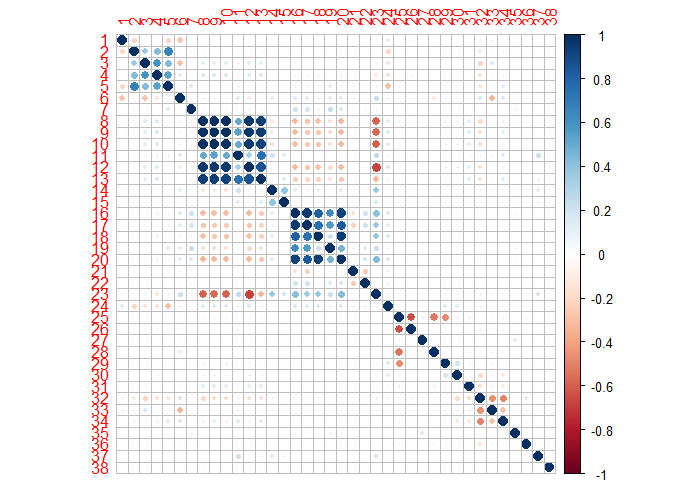
\includegraphics[width=\textwidth]{correlation}

Resultatet af korrelationsanalysen er vist i et korrelationsplot. Resultatet af 
Korrelationsanalysen viser at der er en stor positiv korrelation mellem den fremskrevne
kvadratmeter pris og den vægtede gennemsnitspris for de nærmeste naboer. Der er desuden også 
an større positiv sammenhæng mellem antallet af værelser og boligarealet. 
Disse to positive sammenhænge giver logik rigtig god mening. Salgspriser er i høj grad styret af
det område som ejendommen ligger i. Ligger ejendommen i et dyrt område, vil naboerne blive solgt
til høje handelspriser og det samme vil højst sandsynligt også gælde for den specifikke ejendom. 
Samtidig vil der typisk også være flere væresler jo større boligareal en ejendommene har. 

Som en del af PCA udregnes herefter Singular Value Decomposition (SVD).
De første 16 principal components kan forklare 90\% af variationen i data. For at kommme over 95\%
skal man have de 18 første komponenter. Ud af de i alt 23 mulige komponenter er det med dette data
ikke muligt at reducerer mange komponenter væk uden også at miste variation i data. 

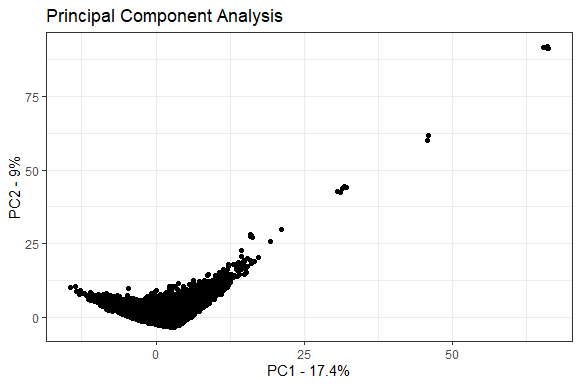
\includegraphics[width=\textwidth]{pca_pc1pc2_plot}


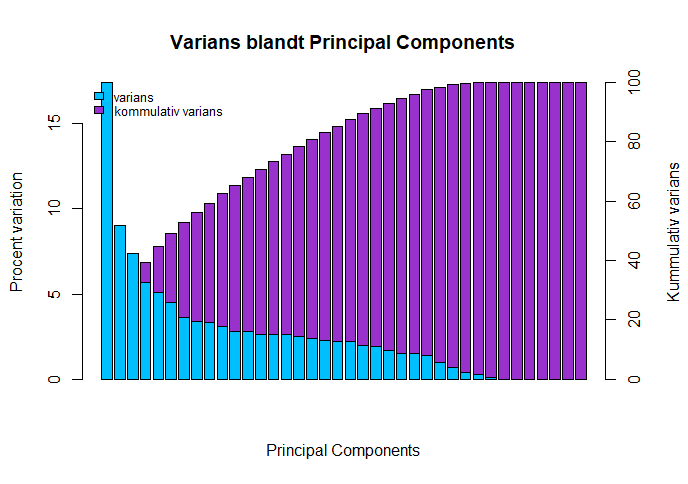
\includegraphics[width=\textwidth]{pca_variation_pct_variation_cummulativt}

Ved at have antallet af komponenter som er mindre end antallet af attributter i ens datasæt bliver
information tabt, og hvorvidt man med fordel kan bruge PCA skal bestemmes ud fra den pågældende
problemstilling. I den videre opgave har jeg valgt at gå videre med mit originale datasæt som det
så ud før PCA. 

\chapter{Part II- Supervised learning}

\section{Regression - part A}
I 2 del er formålet at bruge det rensede data fra del 1 til at forudsige fremskrevne 
kvadratmeterpriser ud fra forskellige variable. Til dette formål vil jeg træne en lineær 
regressionsmodel, da den afhængige variabel "fremskreven kvadratmeterpris" er en numerisk variabel.
I det tilfælde af at det havde været en diskret variabel ville en klassifikationsmodel være blevet
brugt i stedet.
Håbet med denne regressionsanalyse er at man ud fra relativt få variable og en relativt simpel
model vil kunne forudsige ejendomspriserne. 
Forud for regressionsanalysen er data blevet tranformeret. For faktorvariablene tagtype og
vægmateriale har jeg valgt at tranformere med en one-of-k transformering. Herefter er alle
attributter blevet standardiseret, således at de har en gennemsnit på 0 og en standardafvigelse på
1. 

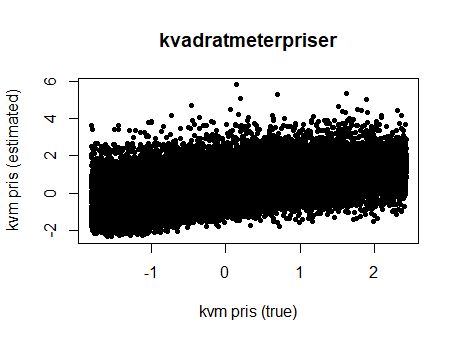
\includegraphics[width=\textwidth]{linear_plot_1}

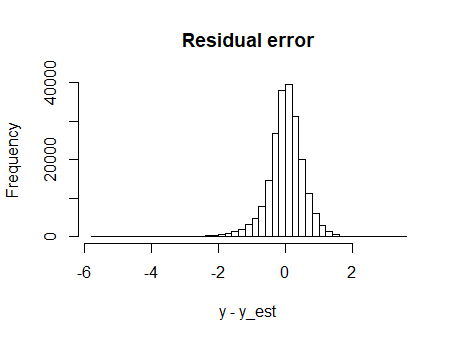
\includegraphics[width=\textwidth]{linear_plot_2}

I en multivariate lineær regressionsmodel kan man ikke på samme måde plotte den fittede model på
det todimensionelle plot. Her kan man i stedet estimerer hvor godt modellen fitter til data ved at
minimere summen af de kvadrerede afvigelser (RSS). 
Der findes flere forskellige typer af algoritmer hvis formål er at finde de parametre/vægte som
laver det bedste fit til data ved at minimerer 'cost'. 

Overfitting er når den trænede model er så god til at forudsige det data den er trænet på at den
ikke kun fanger tendenserne i data men at den også fanger støj. For at undgå at den trænede model
overfitter kan man bl.a. bruge metoden Krydsvalidering. Ved krydsvalidering opdeles data i to
mindre datasæt. Et datasæt som der trænes på og et datasæt som modellen testes på. Selve
opsplitningen i test og træingsdata kan gøres flere gange.

Når modellen er trænet kan man ud fra modellen koefficient estimater se hvor meget de enkelte
parametre bidrager med hvis værdien for den pågældende parameter øges. 
I tilfælde af at de uafhængige variable som indgår i modellen er korrelerede kan estimaterne være
svære at forklare, fordi noget af effekten indirekte ligger i den korrelerede parameter. Dette
påvirker dog ikke nødvendigvis selve prædiktionen. 

I tilfælde at at ens variable ikke er er additive kan man med fordel kigge på interaktionerne
mellem to variable. Dette er endnu en måde at få et bedre fit.

For at undgå overfitting kan man lægge vægte til hver af coefficienterne i modellen som gør at hver enkel variabel får mindre betydning for fittet. Disse vægte kan kontrolleres af lambda. 
Jo større lambda er jo mere straf vil coefficenterne få og jo mindre betyding vil hver variabel have

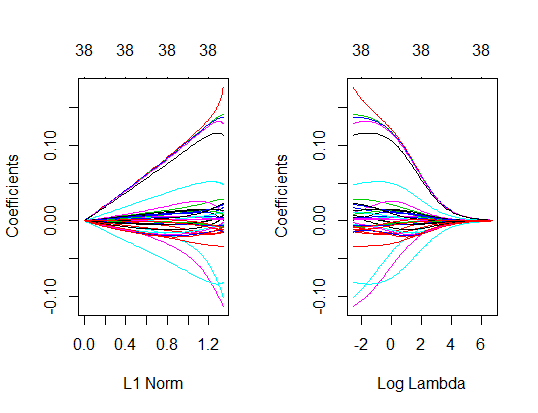
\includegraphics[width=\textwidth]{glmnet_plot}

For at finde den optimale strafværdi kan man tage udgangspunkt i den "mean-squared error" som fittet med den pågældende lambda giver. 
Formålet er her at vælge en lambda værdi hvor man minimerer MSE (mean squared error). 

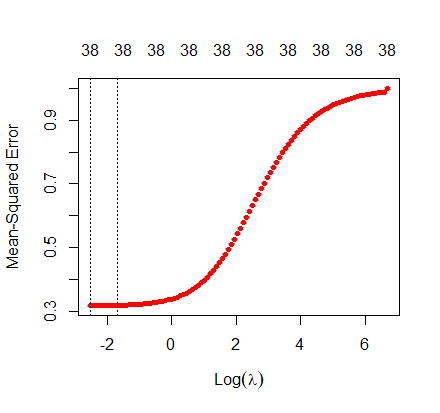
\includegraphics[width=\textwidth]{glmnet_mse}


\chapter{Bilag 1 - Attribut oversigt}
Tabellen nedenfor viser de forskellige typer attributter der er til rådighed i data:
\begin{Schunk}
\begin{Soutput}
# A tibble: 126 x 1
    typer$attributes           $descrete_conti~ $attribute_type $attribute_class
    <fct>                      <chr>            <chr>           <chr>           
  1 aux.adresse.etrs89koordin~ descrete         interval        numeric         
  2 aux.adresse.etrs89koordin~ descrete         interval        numeric         
  3 aux.ice_info.adresse.afst~ descrete         ratio           numeric         
  4 aux.ice_info.adresse.afst~ descrete         ratio           numeric         
  5 aux.ice_info.adresse.afst~ descrete         ratio           numeric         
  6 aux.ice_info.adresse.afst~ descrete         ratio           numeric         
  7 aux.ice_info.adresse.afst~ descrete         ratio           numeric         
  8 aux.ice_info.adresse.afst~ descrete         ratio           numeric         
  9 aux.ice_info.adresse.afst~ descrete         ratio           numeric         
 10 aux.ice_info.adresse.afst~ descrete         ratio           numeric         
 11 aux.ice_info.adresse.afst~ descrete         ratio           numeric         
 12 aux.ice_info.adresse.afst~ descrete         ratio           numeric         
 13 aux.ice_info.adresse.afst~ descrete         ratio           numeric         
 14 aux.ice_info.adresse.afst~ descrete         ratio           numeric         
 15 aux.ice_info.adresse.afst~ descrete         ratio           numeric         
 16 aux.ice_info.adresse.afst~ descrete         ratio           numeric         
 17 aux.ice_info.adresse.afst~ descrete         ratio           numeric         
 18 aux.ice_info.adresse.afst~ descrete         ratio           numeric         
 19 aux.ice_info.adresse.afst~ descrete         ratio           numeric         
 20 aux.ice_info.adresse.afst~ descrete         ratio           numeric         
 21 aux.ice_info.adresse.afst~ descrete         ratio           numeric         
 22 aux.ice_info.adresse.afst~ descrete         ratio           numeric         
 23 aux.ice_info.adresse.afst~ descrete         ratio           numeric         
 24 aux.ice_info.adresse.afst~ descrete         ratio           numeric         
 25 aux.ice_info.adresse.afst~ descrete         ratio           numeric         
 26 aux.ice_info.adresse.afst~ descrete         ratio           numeric         
 27 aux.ice_info.adresse.afst~ descrete         ratio           numeric         
 28 aux.ice_info.adresse.afst~ descrete         ratio           numeric         
 29 aux.ice_info.adresse.afst~ descrete         ratio           numeric         
 30 aux.ice_info.adresse.afst~ descrete         ratio           numeric         
 31 aux.ice_info.adresse.afst~ descrete         ratio           numeric         
 32 aux.ice_info.adresse.afst~ descrete         ratio           numeric         
 33 aux.ice_info.adresse.area~ descrete         ratio           numeric         
 34 aux.ice_info.adresse.udsi~ descrete         ratio           integer         
 35 aux.ice_info.adresse.udsi~ descrete         ratio           numeric         
 36 aux.ice_info.adresse.udsi~ descrete         ratio           numeric         
 37 aux.ice_info.adresse.udsi~ descrete         ratio           integer         
 38 aux.ice_info.adresse.udsi~ descrete         ratio           numeric         
 39 aux.ice_info.bygning.etag~ descrete         ratio           integer         
 40 aux.ice_info.bygning.etag~ descrete         ratio           integer         
 41 aux.ice_info.bygning.etag~ descrete         ratio           integer         
 42 aux.ice_info.bygning.etag~ descrete         ratio           integer         
 43 aux.ice_info.bygning.etag~ descrete         ratio           integer         
 44 aux.ice_info.byzoneareal_~ descrete         ratio           integer         
 45 aux.ice_info.landzonearea~ descrete         ratio           integer         
 46 aux.ice_info.sommerhuszon~ descrete         ratio           integer         
 47 aux.ice_info.jordstykker.~ descrete         ratio           integer         
 48 aux.ice_info.jordstykker.~ descrete         ratio           integer         
 49 bolig_alder                descrete         ratio           integer         
 50 bolig_areal                descrete         ratio           numeric         
 51 bygning.antaletager        descrete         interval        integer         
 52 bygning.arealindbyggetcar~ descrete         ratio           integer         
 53 bygning.arealindbyggetgar~ descrete         ratio           integer         
 54 bygning.bebyggetareal      descrete         ratio           integer         
 55 bygning.bygningenssamlede~ descrete         ratio           integer         
 56 bygning.bygningenssamlede~ descrete         ratio           integer         
 57 bygning.omtilbygningsaar   descrete         interval        integer         
 58 bygning.opfoerelsesaar     descrete         interval        integer         
 59 bygning.samletbygningsare~ descrete         ratio           integer         
 60 enhed.antalbadevaerelser   descrete         ratio           integer         
 61 enhed.antalvaerelser       descrete         ratio           integer         
 62 enhed.antalvandskylledeto~ descrete         ratio           integer         
 63 enhed.arealtilbeboelse     descrete         ratio           integer         
 64 enhed.arealtilerhverv      descrete         ratio           integer         
 65 enhed.enhedenssamledeareal descrete         ratio           integer         
 66 etage.arealafudnyttetdela~ descrete         ratio           integer         
 67 etage.etagensadgangsareal  descrete         ratio           integer         
 68 etage.kaelderareal         descrete         ratio           integer         
 69 EV_NN_M2                   descrete         interval        numeric         
 70 ice_info.min_koteletratio~ continous        interval        numeric         
 71 NN_m2pris_mean             ""               ""              numeric         
 72 NN_m2pris_median           ""               ""              numeric         
 73 NN_m2pris_std              ""               ""              numeric         
 74 NN_m2pris_min              ""               ""              numeric         
 75 NN_m2pris_max              ""               ""              numeric         
 76 NN_m2pris_skewness         ""               ""              numeric         
 77 NN_m2pris_kurtosis         ""               ""              numeric         
 78 NN_afstand_mean            ""               ""              numeric         
 79 NN_afstand_median          ""               ""              numeric         
 80 NN_afstand_std             ""               ""              numeric         
 81 NN_afstand_min             ""               ""              numeric         
 82 NN_afstand_max             ""               ""              numeric         
 83 NN_afstand_skewness        ""               ""              numeric         
 84 NN_afstand_kurtosis        ""               ""              numeric         
 85 NN_m2pris_stdrel           ""               ""              numeric         
 86 ombyg_alder                descrete         interval        numeric         
 87 aux.adresse.etage          descrete         nomial          character       
 88 aux.adresse.regionskode    descrete         nomial          integer         
 89 aux.ice_info.bb_anvendels~ descrete         ratio           integer         
 90 aux.ice_info.bb_anvendels~ descrete         ratio           integer         
 91 aux.ice_info.bb_anvendels~ descrete         ratio           integer         
 92 aux.ice_info.bb_anvendels~ descrete         ratio           integer         
 93 aux.ice_info.bb_anvendels~ descrete         ratio           integer         
 94 aux.ice_info.bb_anvendels~ descrete         ratio           integer         
 95 aux.ice_info.bb_anvendels~ descrete         ratio           integer         
 96 aux.ice_info.bb_anvendels~ descrete         ratio           integer         
 97 ice_info.bb_per_delgrund   descrete         ratio           integer         
 98 ice_info.en_per_delgrund   descrete         ratio           integer         
 99 ice_info.et_per_delgrund   descrete         ratio           integer         
100 ice_info.js_per_delgrund   descrete         ratio           integer         
101 bygning.afloebsforhold     descrete         nomial          character       
102 bygning.bygningensanvende~ descrete         nomial          integer         
103 bygning.opvarmningsmiddel  descrete         nomial          character       
104 bygning.supplerendevarme   descrete         nomial          character       
105 bygning.tagdaekningsmater~ descrete         nomial          character       
106 bygning.vandforsyning      descrete         nomial          integer         
107 bygning.varmeinstallation  descrete         nomial          character       
108 bygning.ydervaeggensmater~ descrete         nomial          character       
109 ejendomsgruppe             descrete         nomial          character       
110 enhed.badeforhold          descrete         nomial          character       
111 enhed.energiforsyning      descrete         nomial          character       
112 enhed.enhedensanvendelse   descrete         nomial          integer         
113 enhed.koekkenforhold       descrete         nomial          character       
114 enhed.opvarmningsmiddel    descrete         nomial          character       
115 enhed.supplerendevarme     descrete         nomial          character       
116 enhed.toiletforhold        descrete         nomial          character       
117 enhed.varmeinstallation    descrete         nomial          character       
118 etage.bygningensetagebete~ descrete         nomial          character       
119 region_nr                  descrete         nomial          integer         
120 aux.vurbenyttelseskode     descrete         nomial          character       
121 fremskreven_pris           continous        interval        numeric         
122 fremskreven_pris_M2        continous        interval        numeric         
123 aux.ice_info.adresse.afst~ descrete         ratio           numeric         
124 aux.ice_info.adresse.afst~ descrete         ratio           numeric         
125 aux.ice_info.adresse.afst~ descrete         ratio           numeric         
126 aux.ice_info.adresse.afst~ descrete         ratio           numeric         
\end{Soutput}
\end{Schunk}

\chapter{Bilag 2 - Manglende værdier}
Tabellen nedenfor viser antallet af manglende værdier i rådata:
\begin{Schunk}
\begin{Soutput}
# A tibble: 126 x 1
    manglende$attributter                      $missing_values $pct_missing_val~
    <fct>                                                <int>             <dbl>
  1 aux.adresse.etage                                   305691            100   
  2 enhed.supplerendevarme                              304896             99.7 
  3 enhed.opvarmningsmiddel                             304723             99.7 
  4 enhed.varmeinstallation                             304004             99.4 
  5 aux.ice_info.adresse.afstand_mellem_soe             280109             91.6 
  6 bygning.afloebsforhold                              212174             69.4 
  7 aux.ice_info.adresse.afstand_lille_soe              172476             56.4 
  8 bygning.supplerendevarme                            170476             55.8 
  9 bygning.opvarmningsmiddel                           153857             50.3 
 10 enhed.energiforsyning                               141739             46.4 
 11 aux.ice_info.adresse.udsigtslinjer_hav                8573              2.8 
 12 aux.ice_info.adresse.udsigtslaengde_samlet            8573              2.8 
 13 aux.ice_info.adresse.udsigtslinjer_soe                8573              2.8 
 14 fremskreven_pris_M2                                   3410              1.12
 15 fremskreven_pris                                      3390              1.11
 16 enhed.badeforhold                                     3053              1   
 17 enhed.toiletforhold                                   3054              1   
 18 bygning.varmeinstallation                             2983              0.98
 19 enhed.koekkenforhold                                  2979              0.97
 20 bygning.tagdaekningsmateriale                         2203              0.72
 21 bygning.ydervaeggensmateriale                         2203              0.72
 22 aux.vurbenyttelseskode                                1611              0.53
 23 aux.adresse.etrs89koordinatnord                        809              0.26
 24 aux.adresse.etrs89koordinatoest                        809              0.26
 25 EV_NN_M2                                               809              0.26
 26 NN_m2pris_mean                                         809              0.26
 27 NN_m2pris_median                                       809              0.26
 28 NN_m2pris_std                                          809              0.26
 29 NN_m2pris_min                                          809              0.26
 30 NN_m2pris_max                                          809              0.26
 31 NN_m2pris_skewness                                     809              0.26
 32 NN_m2pris_kurtosis                                     809              0.26
 33 NN_afstand_mean                                        809              0.26
 34 NN_afstand_median                                      809              0.26
 35 NN_afstand_std                                         809              0.26
 36 NN_afstand_min                                         809              0.26
 37 NN_afstand_max                                         809              0.26
 38 NN_afstand_skewness                                    809              0.26
 39 NN_afstand_kurtosis                                    809              0.26
 40 NN_m2pris_stdrel                                       809              0.26
 41 aux.adresse.regionskode                                809              0.26
 42 ice_info.bb_per_delgrund                                33              0.01
 43 ice_info.en_per_delgrund                                33              0.01
 44 ice_info.et_per_delgrund                                33              0.01
 45 ice_info.js_per_delgrund                                33              0.01
 46 aux.ice_info.adresse.afstand_kyst                        0              0   
 47 aux.ice_info.adresse.afstand_lokalvej                    0              0   
 48 aux.ice_info.adresse.afstand_trafikvej_fo~               0              0   
 49 aux.ice_info.adresse.afstand_trafikvej_ge~               0              0   
 50 aux.ice_info.adresse.afstand_motorvej_mot~               0              0   
 51 aux.ice_info.adresse.afstand_jernbane_hov~               0              0   
 52 aux.ice_info.adresse.afstand_jernbane_any                0              0   
 53 aux.ice_info.adresse.afstand_jernbane_lok~               0              0   
 54 aux.ice_info.adresse.afstand_jernbane_met~               0              0   
 55 aux.ice_info.adresse.afstand_jernbane_reg~               0              0   
 56 aux.ice_info.adresse.afstand_jernbane_reg~               0              0   
 57 aux.ice_info.adresse.afstand_jernbane_s_b~               0              0   
 58 aux.ice_info.adresse.afstand_stor_skov                   0              0   
 59 aux.ice_info.adresse.afstand_lille_skov                  0              0   
 60 aux.ice_info.adresse.afstand_lokalnet_hoe~               0              0   
 61 aux.ice_info.adresse.afstand_regionalnet_~               0              0   
 62 aux.ice_info.adresse.afstand_transmission~               0              0   
 63 aux.ice_info.adresse.afstand_lille_vandlo~               0              0   
 64 aux.ice_info.adresse.afstand_mellem_vandl~               0              0   
 65 aux.ice_info.adresse.afstand_stort_vandlo~               0              0   
 66 aux.ice_info.adresse.afstand_ukendt_vandl~               0              0   
 67 aux.ice_info.adresse.afstand_station_metro               0              0   
 68 aux.ice_info.adresse.afstand_station_s_tog               0              0   
 69 aux.ice_info.adresse.afstand_station_tog                 0              0   
 70 aux.ice_info.adresse.afstand_stor_soe                    0              0   
 71 aux.ice_info.adresse.afstand_lille_vindmo~               0              0   
 72 aux.ice_info.adresse.afstand_mellem_vindm~               0              0   
 73 aux.ice_info.adresse.afstand_stor_vindmoe~               0              0   
 74 aux.ice_info.adresse.areal_samlet_skov                   0              0   
 75 aux.ice_info.adresse.udsigtslaengde_hav                  0              0   
 76 aux.ice_info.adresse.udsigtslaengde_soe                  0              0   
 77 aux.ice_info.bygning.etager.arealaflovlig~               0              0   
 78 aux.ice_info.bygning.etager.arealafudnytt~               0              0   
 79 aux.ice_info.bygning.etager.etagensadgang~               0              0   
 80 aux.ice_info.bygning.etager.kaelderareal                 0              0   
 81 aux.ice_info.bygning.etager.samletarealaf~               0              0   
 82 aux.ice_info.byzoneareal_opsummeret_delj                 0              0   
 83 aux.ice_info.landzoneareal_opsummeret_delj               0              0   
 84 aux.ice_info.sommerhuszoneareal_opsummere~               0              0   
 85 aux.ice_info.jordstykker.registreretareal~               0              0   
 86 aux.ice_info.jordstykker.vejareal                        0              0   
 87 bolig_alder                                              0              0   
 88 bolig_areal                                              0              0   
 89 bygning.antaletager                                      0              0   
 90 bygning.arealindbyggetcarport                            0              0   
 91 bygning.arealindbyggetgarage                             0              0   
 92 bygning.bebyggetareal                                    0              0   
 93 bygning.bygningenssamledeboligareal                      0              0   
 94 bygning.bygningenssamledeerhvervsareal                   0              0   
 95 bygning.omtilbygningsaar                                 0              0   
 96 bygning.opfoerelsesaar                                   0              0   
 97 bygning.samletbygningsareal                              0              0   
 98 enhed.antalbadevaerelser                                 0              0   
 99 enhed.antalvaerelser                                     0              0   
100 enhed.antalvandskylledetoiletter                         0              0   
101 enhed.arealtilbeboelse                                   0              0   
102 enhed.arealtilerhverv                                    0              0   
103 enhed.enhedenssamledeareal                               0              0   
104 etage.arealafudnyttetdelaftagetage                       0              0   
105 etage.etagensadgangsareal                                0              0   
106 etage.kaelderareal                                       0              0   
107 ice_info.min_koteletratiobuff250                         0              0   
108 ombyg_alder                                              0              0   
109 aux.ice_info.bb_anvendelse_0                             0              0   
110 aux.ice_info.bb_anvendelse_910                           0              0   
111 aux.ice_info.bb_anvendelse_920                           0              0   
112 aux.ice_info.bb_anvendelse_930                           0              0   
113 aux.ice_info.bb_anvendelse_940                           0              0   
114 aux.ice_info.bb_anvendelse_950                           0              0   
115 aux.ice_info.bb_anvendelse_960                           0              0   
116 aux.ice_info.bb_anvendelse_970                           0              0   
117 bygning.bygningensanvendelse                             0              0   
118 bygning.vandforsyning                                    0              0   
119 ejendomsgruppe                                           0              0   
120 enhed.enhedensanvendelse                                 0              0   
121 etage.bygningensetagebetegnelse                          0              0   
122 region_nr                                                0              0   
123 aux.ice_info.adresse.afstand_station_any                 0              0   
124 aux.ice_info.adresse.afstand_soe_any                     0              0   
125 aux.ice_info.adresse.afstand_vandloeb_any                0              0   
126 aux.ice_info.adresse.afstand_hoejspaendin~               0              0   
\end{Soutput}
\end{Schunk}

\end{document}
